\subsubsection{Каскад ОИ}

Является аналогом ОЭ
Принципиальная схема:
\begin{center}
	\begin{figure}[h!]
		\center{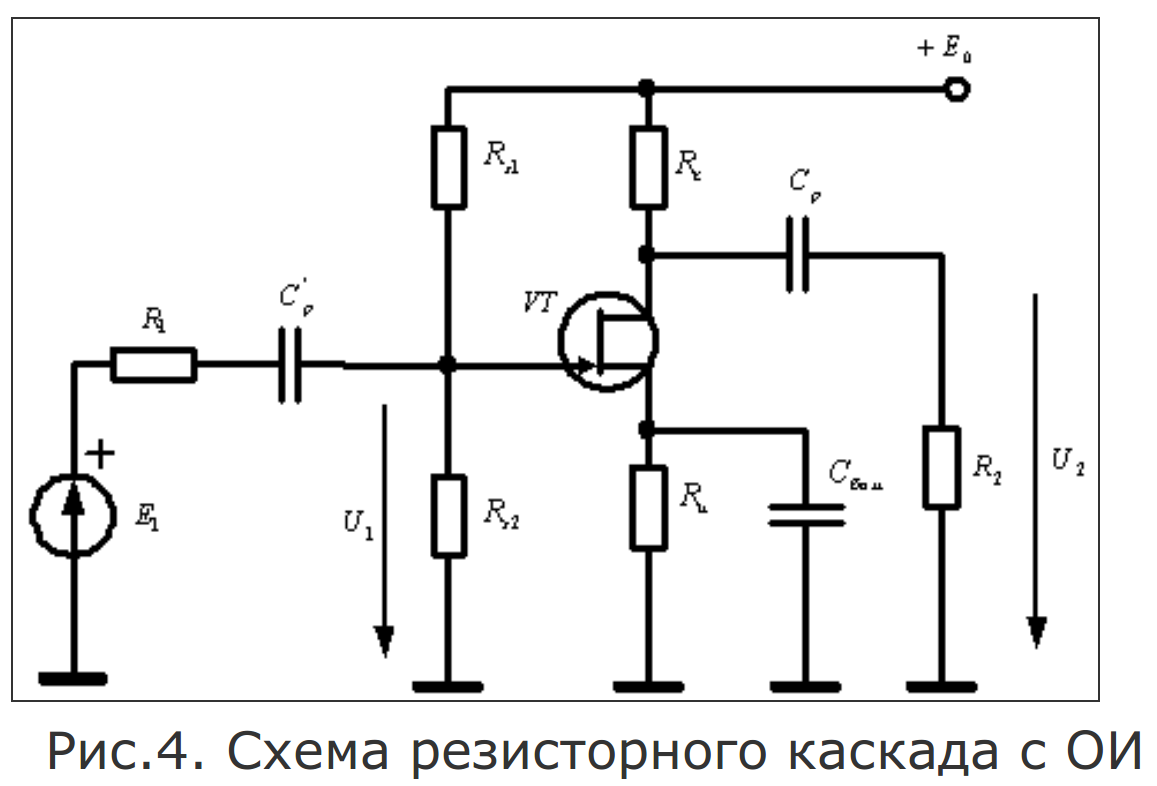
\includegraphics[scale=0.2]{OU.png}}
		\caption{каскад с ОИ}
	\end{figure}
\end{center}

Эквивалентная схема:
\begin{center}
	\begin{figure}[h!]
		\center{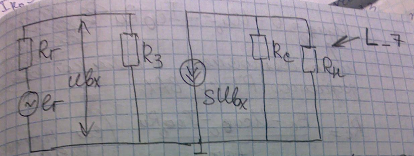
\includegraphics[scale=0.7]{EOU.png}}
		\caption{каскад с ОИ}
	\end{figure}
\end{center}

В схема замещения не учтены резистор $R_u$ и исток $E_c$, т.к. $R_u$ зашутнирован по переменной составляющей конденсатором $C_u$

$X_{C_u}<<R_u\Rightarrow$ потенциал истока по параметрическо составляющей =0

!p-n-переход всегда в обратносмещенном состоянии $\Rightarrow$ ток через резистор $R_3$ не течет. По переменной составляющей тока резистор $R_3$ не должен шунтировать $U_vx \Rightarrow R_3=100kOM...10MOM$ 

По постоянной составляющей $U_z=0$
напряжение U-земля:

$U_u=I_{c_0}R_u(\varphi>0)$

$U_{zu0}=0-U_{u0}=-I_{c_0}R_u$ - напряжение автосмещения, с помощью которой задается РТ на ВАХ.

$R_c=\frac{E_c-U_{cu_0}-I_{c_0}R_u}{I_{c_0}}$(см. принципиальную схема по стрелке сверху-вниз)

$$ \left\{
\begin{aligned}
E_c=U_{Rc}+U_{cu}+U_{Ru}\\
U_{Rc}  = R_cI_{c_0} & &\\
U_{ru} = I_{c_0}R_u & &\\
\end{aligned}
\right. $$

\begin{center}
	\begin{figure}[h!]
		\center{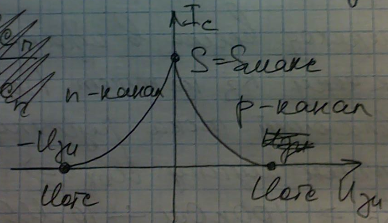
\includegraphics[scale=0.8]{OUgraph1.png}}
	\end{figure}
\end{center}
\pagebreak
\begin{center}
	\begin{figure}[h!]
		\center{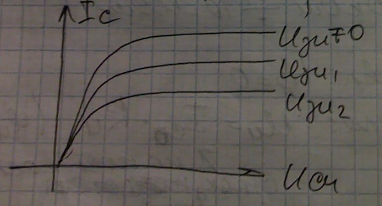
\includegraphics[scale=0.8]{OUgraph2.png}}
	\end{figure}
\end{center}

Входное сопротивление:

$$
R_{vx}=\frac{U_{vx}}{I_{vx}}\approx R_z
$$

Выходное сопротивление:

$R_{vix}=\frac{U_{xx}}{U_{kz}},   U_{xx}=R_cSU_{vx}$

$I_{kz}=SU_{vx}$

$$
R_{vix}\approx R_c\approx \frac1S
$$,что составляет единицы килоОм

Коэффициент усиления по напряжению:
$$
K_u=\frac{U_{vix}}{U_{vx}}=\frac{3U_{vx}(R_c||R_H)}{U_{vx}}=S(R_c||R_H)
$$

Помимо усиления ОИ инвертирует фазу входного сигнала

S - крутизна, $S=\frac{\delta I_c}{\delta U_{zu}}\Rightarrow$ характеризует управляющим свойства затвора

Для пологого участка ВАХ

$S=2b(U_{ots}-U_{zu})$

b - удельная крутизна

$b=\frac{\mu w}{L}$

W - ширина канала

L - длина канала

Выводы:

-каскад облажает очень большим входным сопротивлением.

-Выходное сопротивление определяется сопротивлением резистора в стоковой цепи(около 1-10кОм)

$R_e$ подбирается  так, чтобы не шунтировать входной сигнал и не создавать заметного падения напряжения от протекания через $R_z$ тока утечки обратносмещенного p-n-перехода

Каскад ОС
Аналог эммитерного повторителя(ОК)
Принипиальная схема:
\begin{center}
	\begin{figure}[h!]
		\center{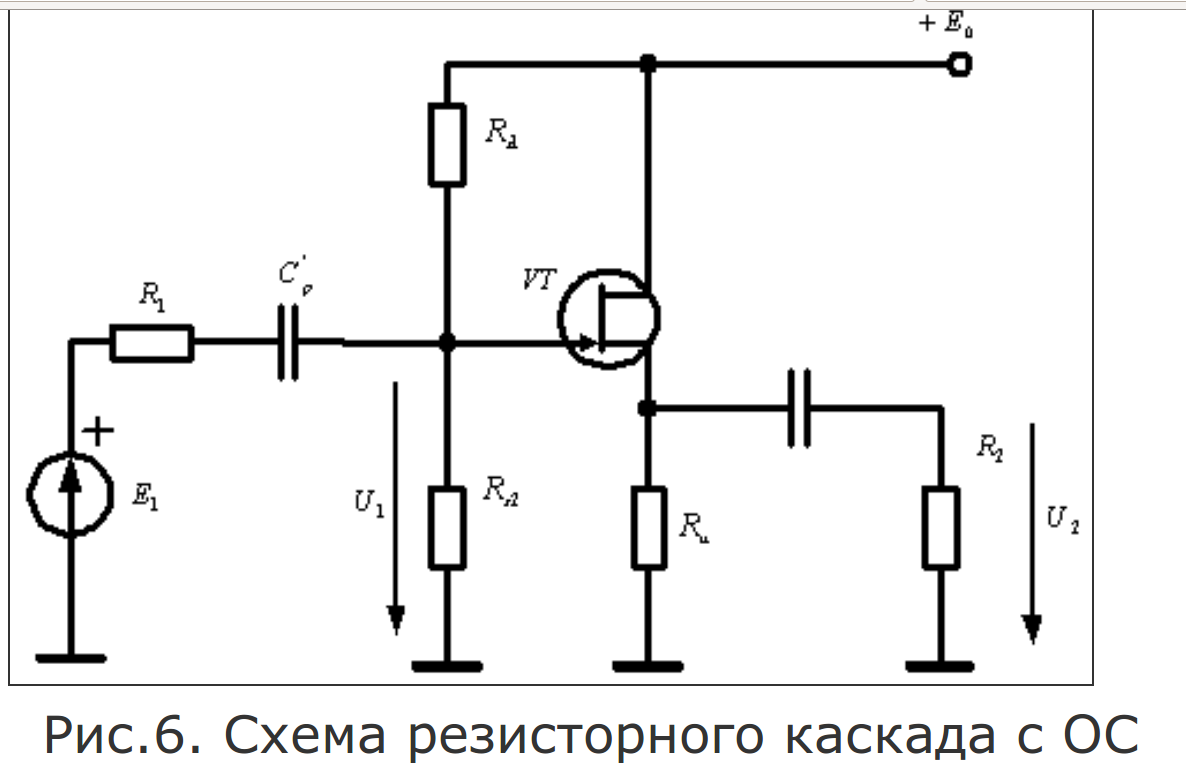
\includegraphics[scale=0.2]{OC.png}}
	\end{figure}
\end{center}
\pagebreak
Эквивалентная схема:
\begin{center}
	\begin{figure}[h!]
		\center{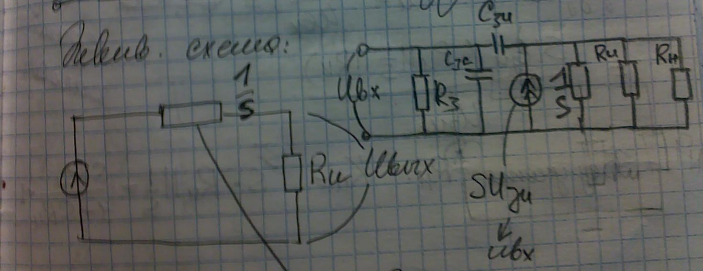
\includegraphics[scale=0.7]{EOC.png}}
	\end{figure}
\end{center}

Входное сопротивление:
$R_{vx}=\frac{U_{vx}}{I_{vix}}$

$S=\frac{dI_c}{dU_zu}$

$r_{dif}=\frac1S$ - дифференциальное сопротивление.

p-n-переход всегда в обратном смещенном состоянии $\Rightarrow$ ток через $R_z$ не течет

$R_{vx}\approx R_z\sim 1MOM$

$R_{vix}$ - определяется при отключенном генераторе и нагрузке

$R_{vix}=\frac{U_{xx}}{I_{kz}}, U_{xx}=(R_H)||\frac1S)SU_{zu}$

$I_{kz}=SU_{zu}\Rightarrow R_{vix}=R_u||\frac1S=\frac{R_u}{1+SR_u}\approx \frac1S$

$$
K_u=\frac{U_{vix}}{U_{vx}}=\frac{SU_{zu}(R_u||frac1S||R_H)}{U_{zu}}
$$

Без учета $R_H$:

$$
K_u=SR_u||\frac1S=\frac{SR_u}{1+SR_u}<1
$$

Каскад ОЗ:

СОНЯ НЕ НАШЛА ВЫВОД ФОРМУЛ!!!!!!!!!!!!!!!!!!!!!!!!!!!!!!!!!!!!!!!!!!!!!!!!!!!!!!!!!!!!!!!!!!!!!!!!!!!!!!!!!!!!!!!!!!!

является аналогом ОБ

\pagebreak
Принципиальная схема:
\begin{center}
	\begin{figure}[h!]
		\center{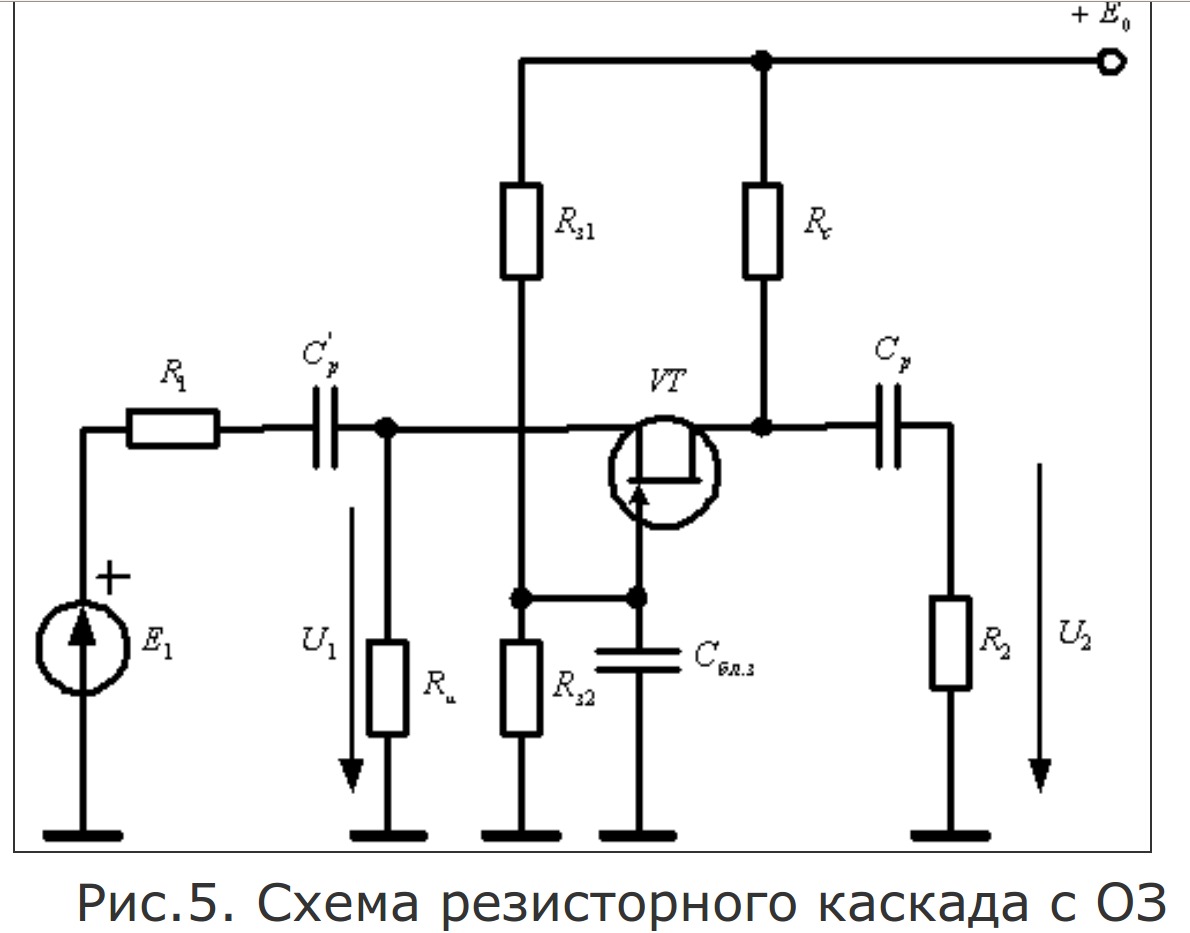
\includegraphics[scale=0.2]{OZ.png}}
	\end{figure}
\end{center}
Эквивалентная схема:
\begin{center}
	\begin{figure}[h!]
		\center{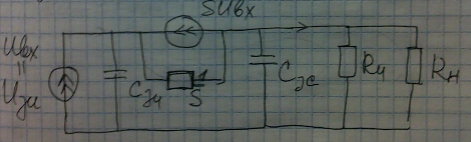
\includegraphics[scale=0.7]{EOZ.png}}
	\end{figure}
\end{center}

Входное сопротивление:
$$
R_{vx}=\frac1S||R_u
$$

$S=\frac{\delta I_c}{\delta U_{zn}}$

$r_{dif}=\frac1S$

Выходное сопротивдение:
$$
R_{vix}=(1+SR_g)R_u
$$
Коэффициент усиления по напряжению:
$$
K_u=\frac{U_{vix}}{U_{vx}}=\frac{SU_{vx}R_u||R_H}{U_{vx}}=S(R_u||R_H)
$$